
\chapter{三次曲面上的二十七条线}
\label{ch:twenty-seven-lines}

\epigraph{在深夜叫醒一位代数几何学家，对他耳语「27」。十有八九，他会答道：「三次曲面上的线。」}{——R.~\trDonagi{}与 R.~\trSmith，[DS]（当然，说的是第 27 页）}

\begin{figure}[htbp]
\centering
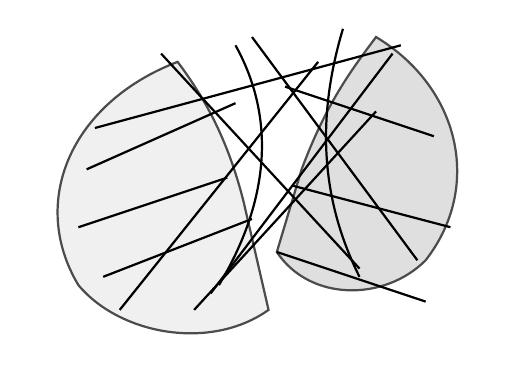
\begin{tikzpicture}[scale=1.05,line width=0.8pt]
  \fill[gray!12,draw=black!70] (2.2,3.9) .. controls (0.9,3.4) and (0.4,2.2) .. (1.0,1.2)
        .. controls (1.5,0.6) and (2.6,0.4) .. (3.3,0.9)
        -- (3.0,2.2) .. controls (2.8,3.0) and (2.5,3.5) .. (2.2,3.9) -- cycle;
  \fill[gray!25,draw=black!70] (4.6,4.2) .. controls (5.6,3.6) and (5.9,2.4) .. (5.2,1.5)
        .. controls (4.7,1.0) and (3.8,1.0) .. (3.4,1.6)
        -- (3.7,2.6) .. controls (4.0,3.4) and (4.3,3.8) .. (4.6,4.2) -- cycle;
  \draw (2.9,4.1) .. controls (3.4,3.2) and (3.3,2.2) .. (2.7,1.2);
  \draw (4.2,4.3) .. controls (3.9,3.3) and (3.9,2.3) .. (4.4,1.3);
  \draw (1.1,2.6) -- (2.9,3.4); \draw (1.0,1.9) -- (2.8,2.5);
  \draw (1.3,1.3) -- (3.1,2.0); \draw (3.5,3.6) -- (5.3,3.0);
  \draw (3.6,2.4) -- (5.5,1.9); \draw (3.4,1.6) -- (5.2,1.0);
  \draw (2.0,4.0) -- (4.4,1.4); \draw (3.1,4.2) -- (5.1,1.5);
  \draw (1.2,3.1) -- (4.9,4.1); \draw (2.4,0.9) -- (4.6,3.3);
  \draw (1.5,0.9) -- (3.9,3.9); \draw (4.8,4.0) -- (2.6,1.1);
\end{tikzpicture}
\caption{Clebsch 三次曲面上的 27 条线。（原书为 Greg Egan 提供的三维渲染图，此处以示意图代替。）}\label{fig:clebsch-27-lines}
\end{figure}

自十九世纪中叶起，几何学家便为「每个光滑三次曲面上都有 27 条线」这一事实，以及这些线的构型所具有的非凡结构而心醉神迷。它们由\trCayley{}与\trSalmon{}于 1849 年发现，被称为现代代数几何的开端，[Do, p.~55]。

之所以有如此多的人被这一事实迷住，是因为它需要一点魔法，而这种魔法又与许多别的事物相通：既有我们已经讨论过的若干基本观念，也有其他优美的经典构造（比如\trPascal{}的「神秘六边形」定理~19.4.4、大多数光滑四次平面曲线有 28 条双切线这一事实、例外李群……），还有现代代数几何的许多主题（形变理论、相交理论、计数几何、算术与丢番图问题……）。对我们来说它将格外令人愉快，因为它用到了我们学过的许多东西。

现在，你已准备好被接纳入 27 条线的秘密会社了。

\textbf{27.0.1. \trhTheorem。}\ ——\ \emph{$\mathbb{P}^3_{\bar{k}}$ 中的每个光滑三次曲面都恰有 27 条线。}

\mbox{定理~27.0.1} 与下述结果紧密相关。

\textbf{27.0.2. \trhTheorem。}\ ——\ \emph{$\bar{k}$ 上的每个光滑三次曲面都\trIsomorphic{}于 $\mathbb{P}^2$ 在六个点处的\trBlowup。}

人们认为这些事实有魔力，理由很多。首先，是「总有 27 条线」这一事实。与计数几何中的大多数问题不同，这里没有「一个一般的三次曲面」「大多数三次曲面」「正确地计数」之类的滑头措辞——就像「每个首一 $d$ 次多项式有 $d$ 个根——只要正确地计数」那样。而且不知何故（我们将会看到如何），恰恰是曲面的光滑性使它得以成立。

其次，有这样的魔力：你总是得到平面在六个点处的\trBlowup（\S27.3）。

第三，是 27 条线那有魔力的关联结构，它与李理论中的 $\mathrm{E}_6$ 相联系。$\mathrm{E}_6$ 的\trWeyl{}群正是这一关联结构的对称群（见\mbox{注记~27.2.5}）。以一种自然的方式，这 27 条线构成 $\mathrm{E}_6$ 的 27 维基础表示的一组基。

\textbf{27.0.3. 本章的结构。}\quad 在本章中，$X$ 将是代数闭域 $\bar{k}$ 上的一条光滑三次曲面。\S27.1 中我们建立一些预备事实。\S27.2 中我们证明\mbox{定理~27.0.1}（在特征 $3$ 之外的范围内）。\S27.3 中我们证明\mbox{定理~27.0.2}。我们在此指出：\S27.3 需要从 \S27.2 那里获得的唯一输入是\mbox{练习~27.2.J}。这可以直接徒手完成（例如见 [Rei1, \S7]、[Be, Thm.~IV.13] 或 [Sh, pp.~246--7]），而\mbox{定理~27.0.2} 借助\mbox{练习~27.3.F} 即可轻易蕴含\mbox{定理~27.0.1}。这样我们其实还有另一条更短的\mbox{定理~27.0.1} 的证明。之所以给出 \S27.2 的论证，理由在于：就我们目前所学而言它是自然的，它让你得以窥见本学科中更广泛使用的一些想法（关键想法是：从一个\trModuliSpace{}到另一个\trModuliSpace{}的态射是有限且平坦的），并且它或许有助于你进一步领会和消化我们已发展出的那些工具。

\textbf{27.0.4. 本章的位置。}\quad 这一主题被放在第 27 章，纯粹是出于数字命理上的原因；它当然可以在第 24 章之后阅读。这是一个特性而非缺陷：你无须读完后面各章的细节也能享受本章。事实上，你或许应该在早得多的阶段就读它，把关键事实当作「黑盒子」，从而在学习那些看似技术性的定义与定理之前，先体会它们的价值。作为一本劲头十足的代数几何导论，这是一个恰如其分的收束，即便你此前尚未覆盖为全部细节正名所需的一切。


\section{预备事实}

由\mbox{必要练习~15.1.C}，四个变量的三次\trForm{}构成一个 $20$ 维\trVectorSpace，于是 $\mathbb{P}^{3}$ 中的三次曲面由 $\mathbb{P}^{19}$ 参数化。设 $\Delta\subset\mathbb{P}^{19}$ 为对应于奇异三次\trHypersurface{}的\trLocus。\mbox{\trBertini{}定理~13.4.2} 表明：光滑三次曲面所在的\trLocus{} $\mathbb{P}^{19}\setminus\Delta$ 在全体三次曲面构成的空间 $\mathbb{P}^{19}$ 中既\trDense{}又\trOpen。

\textbf{27.1.A.（练习）}\quad 证明：任何光滑三次曲面 $X$ 都是「反典范嵌入的」——也就是说，它由完全反\trCanonical\trLinearSystem{} $\mathscr{K}_X^{\vee}$ 所嵌入。提示：\trAdjunctionFormula（\mbox{练习~21.5.B}）。

\textbf{27.1.B.（练习）}\quad 设 $X\subset\mathbb{P}^{3}_{\bar{k}}$ 是一张光滑三次曲面，而 $C$ 是 $X$ 上的一条\trCurve。证明：$C$ 是一条直线，当且仅当 $C$ 是一条 $(-1)$-\trCurve（\mbox{定义~20.2.8}）。提示：仍是\trAdjunctionFormula，或许以\mbox{练习~20.2.B}(a) 的面貌出现；另外还可参\mbox{练习~18.6.K}。

找出\emph{单独一个}域上\emph{单独一张}恰好具有 27 条直线的三次曲面，将会是有用的：

\textbf{27.1.C.（动手练习）}\quad 证明\trFermat{}三次曲面
\[
\tag{27.1.0.1}\label{eq:fermat-cubic-surface}
x_0^{3}+x_1^{3}+x_2^{3}+x_3^{3}=0
\]
在 $\mathbb{P}^{3}_{\mathbb{C}}$ 中恰有 27 条直线，每条都形如
\[
x_0+\omega x_i=x_j+\omega' x_k=0,
\]
其中 $\{1,2,3\}=\{i,j,k\}$，$j<k$，而 $\omega$ 与 $\omega'$ 都是 $1$ 的立方根（可以相同）。这将需要一些蛮力。可能的提示：在相差一个坐标置换的意义下，证明 $\mathbb{P}^{3}$ 中的每条直线都可以写成 $x_0=ax_2+bx_3$，$x_1=cx_2+dx_3$。证明：这条直线落在 \eqref{eq:fermat-cubic-surface} 上，当且仅当
\[
\tag{27.1.0.2}\label{eq:fermat-line-condition}
a^{3}+c^{3}+1=b^{3}+d^{3}+1=a^{2}b+c^{2}d=ab^{2}+cd^{2}=0
\]
再证明：若 $a$、$b$、$c$、$d$ 全都非零，则 \eqref{eq:fermat-line-condition} 无解。

\textbf{27.1.1.}\ \hard\ \textbf{奇异三次曲面在全体三次曲面的参数空间 $\mathbb{P}^{19}$ 中给出一个\trIrreducible\trDivisor{} $\Delta$。}\quad 这段讨论被标上星号，不是因为它难，而是因为本章其余部分并不需要它。尽管如此，它是对我们已学内容的一个漂亮应用，并且预示了 \S27.2 中论证的关键部分。

\mbox{\trBertini{}定理~13.4.2} 表明：全体三次曲面构成的空间 $\mathbb{P}^{19}$ 中光滑三次曲面所在的\trLocus{}既\trDense{}又\trOpen，但该证明还暗示了更多的东西：这个\trLocus{}的\trComplement{} $\Delta$ 具有纯余维数 $1$。我们现在就来证明事情确乎如此，甚至证明这个「\trDiscriminant{}超曲面」$\Delta$ 是\trIrreducible{}的。

\textbf{27.1.D.（练习）}\quad（两小问共用提示：回想\mbox{练习~12.2.N} 的解答。）
（a）定义\trIncidenceCorrespondence{} $Y\subset\mathbb{P}^{19}\times\mathbb{P}^{3}$，它对应于「一张三次曲面 $X$ 连同其上一个\trSingularPoint{} $p\in X$」这份数据。（这是练习的一部分！我们需要的是作为概形的 $Y$，而不只是作为集合的 $Y$。）令 $\mu$ 为\trProjection{} $Y\to\mathbb{P}^{19}$。
\[
\begin{tikzcd}[row sep=2.2em, column sep=3.6em]
& Y \ar[dl, "\mu"] \ar[dr, "\mathbb{P}^{15}\text{-丛}"] & \\
\mathbb{P}^{19} && \mathbb{P}^{3}
\end{tikzcd}
\]
（b）通过把 $Y$ 描述为 $\mathbb{P}^{3}$ 上的一个 $\mathbb{P}^{15}$-丛，证明 $Y$ 是维数为 $18$ 的\trIrreducible{}光滑\trVariety。

\textbf{27.1.E.（练习）}\quad 证明：存在只有一个\trSingularPoint{}的三次曲面。你尽可随意假设 $k$ 是你最喜欢的\trField；这里的要点是让你熟悉几何想法，而不是正特征\trField{}的种种怪癖。（$\operatorname{char}k\neq 2$ 情形的提示：\mbox{练习~13.3.C}。）

\textbf{27.1.F.（练习）}\quad 证明：$\mu(Y)=\Delta$ 是一个余维数为 $1$ 的\trClosed\trIrreducible{}子集。余维数 $1$ 部分的提示：\mbox{练习~12.4.A} 或\mbox{定理~12.4.1}，与\mbox{练习~27.1.E} 结合起来用。

你的论证几乎无须改动即可推广，用以处理 $\mathbb{P}^{n}$ 中次数 $d$ 的\trHypersurface。


\section{每个光滑三次曲面（$\bar{k}$ 上）都有 27 条线}

我们现已准备好证明\mbox{定理~27.0.1}。在到达\mbox{练习~27.2.K}之前，为免分心，我们假设 $\operatorname{char}\bar{k}=0$。不过，即便 $\operatorname{char}\bar{k}\neq 3$，下面的论证也无须改动即可通过。唯一需要的一处检验——也正是对特征加以限制的原因——是\mbox{练习~27.1.C} 在把 $\mathbb{C}$ 换成任何一个这样的 $\bar{k}$ 之后依然成立。

\textbf{27.2.A.（练习）}\quad（两小问共用提示：回想\mbox{练习~12.2.N} 的解答。）
（a）定义\trIncidenceCorrespondence{} $Z\subset\mathbb{P}^{19}\times\mathbb{G}(1,3)$，它对应于「$\mathbb{P}^{3}$ 中含于某张三次曲面 $X$ 的一条直线 $\ell$」这份数据。（与\mbox{练习~27.1.D} 一样，这也是练习的一部分。）令 $\pi$ 为\trProjection{} $Z\to\mathbb{P}^{19}$。
\[
\begin{tikzcd}[row sep=2.2em, column sep=3.6em]
& Z \ar[dl, "\pi"] \ar[dr, "\mathbb{P}^{15}\text{-丛}"] & \\
\mathbb{P}^{19} && \mathbb{G}(1,3)
\end{tikzcd}
\]
（b）通过把 $Z$ 描述为\trGrassmannian{} $\mathbb{G}(1,3)$ 上的一个 $\mathbb{P}^{15}$-丛，证明 $Z$ 是维数为 $19$ 的不可约光滑\trVariety。

\textbf{27.2.B.（练习）}\quad 利用「存在只有有限多条直线的三次曲面」（\mbox{练习~27.1.C}）这一事实，以及态射纤维维数的行为（\mbox{练习~12.4.A} 或\mbox{定理~12.4.1}），证明下述诸条。
（a）每张三次曲面都含有直线，也就是说 $\pi$ 是满射。（提示：证明 $\pi$ 是\trProjective{}的。）
（b）「大多数三次曲面只有有限多条直线」：存在一个\trDense{}\trOpenSubset{} $U\subset\mathbb{P}^{19}$，使得由 $U$ 的\trClosedPoint{}所参数化的那些三次曲面都有条数为正的有限多条直线。（提示：纤维维数的\trUpperSemicontinuous{}性，\mbox{定理~12.4.3}。）

下面这个事实是\mbox{定理~27.0.1} 证明中的关键结果，也是 27 条线的主要奇迹之一：它保证在一张光滑曲面上，这些直线能保持两两相异。它的非正式陈述是：两条线不可能凑到一起而不损伤曲面。这其实是一条\trDeformationTheory{}的结果：我们正在显式地证明，光滑三次曲面中的一条直线没有任何一阶形变。

\textbf{27.2.1. \trhTheorem。}\ ——\ \emph{若 $\ell$ 是一张正则三次曲面 $X$ 中的一条直线，则 $\{\ell\subset X\}$ 是 $\pi\colon Z\to\mathbb{P}^{19}$ 的纤维中的一个\trReduced{}孤立点。}

在证明\mbox{定理~27.2.1} 之前，我们先用它来证明\mbox{定理~27.0.1}。

\textbf{27.2.2.}\ \emph{\mbox{定理~27.0.1} 的证明（假定\mbox{定理~27.2.1}）。}\quad 此时 $\pi$ 是一个\trProjective{}\trMorphism，而由\mbox{定理~27.2.1}，在 $\mathbb{P}^{19}\setminus\Delta$ 之上，$\pi$ 的相对维数为 $0$，从而具有有限的\trFiber。于是，由\mbox{定理~18.1.6}（射影＋有限纤维＝有限），$\pi$ 在 $\mathbb{P}^{19}\setminus\Delta$ 上是有限的。

此外，$Z$ 与 $\mathbb{P}^{19}$ 都（在 $\mathbb{Z}$ 上）光滑且维数为 $19$，而 $\pi\colon Z\to\mathbb{P}^{19}$ 在 $\mathbb{P}^{19}\setminus\Delta$ 上方的\trFiber{}是（几何）既约的点，这仍由\mbox{定理~27.2.1} 得出。再由\mbox{练习~24.8.G}，$\pi$ 在 $\mathbb{P}^{19}\setminus\Delta$ 上是\trEtale{}的（并且，特别地，是\trFlat{}的）。

于是，在 $\mathbb{P}^{19}\setminus\Delta$ 之上，$\pi$ 是一个有限\trFlat{}\trMorphism，从而 $\pi$ 的\trFiber（再次强调，在远离 $\Delta$ 处）总有相同个数的点——「按正确方式计数」（\mbox{注记~24.3.8}）。但由\mbox{定理~27.2.1}，在 $\mathbb{P}^{19}\setminus\Delta$ 的每个\trClosedPoint{}上方，纤维的每个点都以重数 $1$ 计入（这里用到 $k=\bar{k}$）。最后，由\mbox{练习~27.1.C}，\trFermat{}三次曲面给出了一张恰有 27 条直线的正则三次曲面的例子，所以（由于 $\mathbb{P}^{19}\setminus\Delta$ 是\trConnected{}的）我们便证毕了。\hfill$\square$

我们实际上已经证明了：在远离 $\Delta$ 处，$Z\to\mathbb{P}^{19}$ 是一个次数为 $27$ 的有限平展态射。

\textbf{27.2.3.}\ \hard\ \emph{\mbox{定理~27.2.1} 的证明。}\quad 选取射影坐标，使得直线 $\ell$ 在一个特异仿射子集（其坐标记为 $x$、$y$、$z$）中由 $z$-轴给出。（我们使用仿射坐标，是为了帮助看清正在做的事情；尽管如此，这个论证用射影坐标来做会更好。在重读时，你应当把它翻译成一个完全射影的论证。）

\textbf{27.2.C.（练习）}\quad 考虑形如 $(x,y,z)=(a,b,0)+t(a',b',1)$ 的直线（其中 $(a,b,a',b')\in\mathbb{A}^{4}$ 固定，而 $t$ 在 $\mathbb{A}^{1}$ 中变动）。证明：$a$、$b$、$a'$、$b'$ 可以被释读为\trGrassmannian{}的某个标准\trOpenSubset{}上的「通常」坐标（见 \S7.7），并以 $[\ell]$ 为原点。

在\trModuliSpace{}上建立好局部坐标之后，我们就可以进入正题了。设 $f(x,y,z)=0$ 是三次曲面 $X$ 的方程（的仿射版本）。由于 $X$ 包含 $z$-轴 $\ell$，故 $f(x,y,z)\in(x,y)$。更一般地，直线
\[
\tag{27.2.3.1}\label{eq:nearby-line-param}
(x,y,z)=(a,b,0)+t(a',b',1)
\]
含于 $X$，当且仅当 $f(a+ta',\,b+tb',\,t)$ 作为 $t$ 的三次多项式恒为 $0$。这等价于 $a$、$a'$、$b$、$b'$ 的四个方程，分别对应于 $t^{3}$、$t^{2}$、$t$ 与 $1$ 的系数。这比一个单纯的集合论陈述要强：

\textbf{27.2.D.（练习）}\quad 验证：这四个方程是\trSchemeTheoreticFiber（或\trSchemeTheoreticPreimage）$\pi^{-1}([X])$ 的局部方程。

现在我们来到论证的关口，在这里我们要用到 $X$（沿 $\ell$）的正则性。我们有的是一个代数中的精确问题。给定一张由 $f(x,y,z)=0$ 给出的三次曲面 $X$，它含有 $\ell$，而且我们知道 $X$ 是正则的（包括「在无穷远处」，即在 $\mathbb{P}^{3}$ 中）。为了证明 $[\ell]=V(a,a',b,b')$ 是 $\pi$ 的纤维中的一个\trReduced{}孤立点，我们在环 $k[a,a',b,b']/(a,a',b,b')^{2}$ 中工作，也就是说，我们施加方程

\begin{figure}[htbp]
\centering
\begin{tikzpicture}[scale=1.0,line width=0.7pt]
  \draw (0.6,3.4) -- (4.6,3.7) -- (6.2,2.9) -- (2.2,2.6) -- cycle;
  \node[anchor=west] at (5.35,2.72) {$z=1$};
  \draw (0.2,1.0) -- (4.2,1.3) -- (5.8,0.5) -- (1.8,0.2) -- cycle;
  \node[anchor=west] at (4.85,0.32) {$z=0$};
  \fill (2.6,3.06) circle (1.2pt);
  \node[anchor=south east] at (2.62,3.08) {$(0,0,1)$};
  \fill (4.4,3.2) circle (1.2pt);
  \node[anchor=south west] at (4.42,3.22) {$(a+a',\,b+b',\,1)$};
  \fill (2.2,0.86) circle (1.2pt);
  \node[anchor=north east] at (2.22,0.84) {$(0,0,0)$};
  \fill (3.4,0.95) circle (1.2pt);
  \node[anchor=north west] at (3.42,0.93) {$(a,b,0)$};
  \draw (2.6,3.06) -- (2.2,0.86);
  \node[anchor=east] at (2.1,2.0) {$\ell$};
  \draw (4.4,3.2) -- (3.4,0.95);
  \node[anchor=west] at (4.15,2.1) {「附近的直线」};
\end{tikzpicture}
\caption{「$\ell$ 附近的直线」所成空间的参数：以它们与 $z=0$ 平面和 $z=1$ 平面相交的位置表出。（依原书手绘图重绘。）}\label{fig:lines-near-ell}
\end{figure}

\[
\tag{27.2.3.2}\label{eq:nearby-line-square-zero}
a^{2}=aa'=\cdots=(b')^{2}=0,
\]
并试图由此证明 $a=a'=b=b'=0$。（理解「我们为何令 $(a,a',b,b')^{2}=0$」是至关重要的。你也可以从所涉函数的导数这一角度来解读这个论证——归根结底，这可以理解为忘掉高阶信息、只记住相关变量中的一次项；参看\mbox{练习~13.1.I}。关于以导数语言对这一计算的描述，见 [Mu6, \S8D]。）

设 $f(x,y,z)=c_{x^{3}}x^{3}+c_{x^{2}y}x^{2}y+\cdots+c_{1}1=0$，其中 $c_{x^{3}},\,c_{x^{2}y},\,\cdots\in\bar{k}$。由于 $\ell\subset X$，即 $f\in(x,y)$，我们有 $c_{1}=c_{z}=c_{z^{2}}=c_{z^{3}}=0$。现在把 \eqref{eq:nearby-line-param} 代入 $f$，再施加 \eqref{eq:nearby-line-square-zero}。$f$ 的系数中，只有那些恰含一个 $x$ 或一个 $y$ 的单项式的系数存活下来：
\begin{multline*}
c_{x}(a+a't)+c_{xz}(a+a't)t+c_{xz^{2}}(a+a't)t^{2} \\
+c_{y}(b+b't)+c_{yz}(b+b't)t+c_{yz^{2}}(b+b't)t^{2} \\
=\;(a+a't)\bigl(c_{x}+c_{xz}t+c_{xz^{2}}t^{2}\bigr)+(b+b't)\bigl(c_{y}+c_{yz}t+c_{yz^{2}}t^{2}\bigr)
\end{multline*}
被要求作为 $t$ 的多项式恒为 $0$。（回想 $c_{x},\dots,c_{yz^{2}}$ 是 $\bar{k}$ 中固定的元素。）为方便计，令 $C_{x}(t)=c_{x}+c_{xz}t+c_{xz^{2}}t^{2}$ 与 $C_{y}(t)=c_{y}+c_{yz}t+c_{yz^{2}}t^{2}$。

现在，$X$ 在 $(0,0,0)$ 处正则，当且仅当 $c_{x}$ 与 $c_{y}$ 不全为零（因为 $c_{z}=0$）。更一般地，$X$ 在 $(0,0,t_{0})$ 处正则，当且仅当 $c_{x}+c_{xz}t_{0}+c_{xz^{2}}t_{0}^{2}=C_{x}(t_{0})$ 与 $c_{y}+c_{yz}t_{0}+c_{yz^{2}}t_{0}^{2}=C_{y}(t_{0})$ 不全为零。你应当能够很快检验：$X$ 在 $\ell$ 「在无穷远处」的那一点处正则，当且仅当 $c_{xz^{2}}$ 与 $c_{yz^{2}}$ 不全为零。我们把这一点总结如下：$X$ 在 $\ell$ 的每一点处都正则，当且仅当两个二次多项式 $C_{x}(t)$ 与 $C_{y}(t)$ 没有公共根——包括「在无穷远处」。

现在我们就用它，在 $(a+a't)C_{x}(t)+(b+b't)C_{y}(t)\equiv 0$ 的条件下迫使 $a=a'=b=b'=0$。

我们先处理 $C_{x}$ 与 $C_{y}$ 有两个相异根、且两根都有限的特殊情形（即 $c_{xz^{2}}$ 与 $c_{yz^{2}}$ 非零）。设 $t_{0}$ 与 $t_{1}$ 是 $C_{x}(t)$ 的根；把 $t_{0}$ 与 $t_{1}$ 代入 $(a+a't)C_{x}(t)+(b+b't)C_{y}(t)$，便得到 $b+b't_{0}=0$ 与 $b+b't_{1}=0$，从而 $b=b'=0$。同理，$a=a'=0$。

\textbf{27.2.E.（练习）}\quad 处理余下的情形，以完成\mbox{定理~27.2.1} 的证明。（这件事可以做得相当巧妙。例如，你或许能够重新选取坐标，使得 $C_{x}$ 与 $C_{y}$ 的根都是有限的。）\hfill$\square$

\textbf{27.2.4. 直线的构型。}\quad 所谓三次曲面上的「直线构型」，指的是「27 条线中哪些对相交」这份数据。在\trFermat{}三次曲面这一特殊情形（\mbox{练习~27.1.C}），我们不难把它算出来。（利用 $X$ 作为 $\mathbb{P}^{2}$ 的\trBlowup{}的描述，或许更具启发性；见\mbox{练习~27.3.F}。）我们现在来证明：对全体光滑三次曲面，这个构型都是「相同的」（在恰当的解读之下）。

\textbf{27.2.F.（练习）}\quad 构造一个次数为 $27!$ 的有限平展映射 $W\to\mathbb{P}^{19}\setminus\Delta$，它把一张三次曲面连同 27 条相异直线的一个\emph{有序清单}一同参数化。提示：令 $W'$ 为 $Z$ 在 $\mathbb{P}^{19}\setminus\Delta$ 上的第 $27$ 个\textbf{纤维幂}（fibered power），把它释读为对「一张三次曲面连同 27 条直线的有序清单（诸线不必相异）」的参数化。令 $W$ 为诸线相异处对应的子集，证明 $W$ 在 $W'$ 中既开又闭，从而是 $W'$ 的若干连通分量之并。另一种在 $W'$ 中辨认出 $W$ 的办法（这种做法或许能推广到\mbox{练习~27.2.H}）：给「对每一对 $i,j$，『$\ell_i\cdot\ell_j$』是 $W'$ 上的局部常值函数」这一事实赋予意义，于是这些函数对一切 $i\neq j$ 都取正值的位置既开又闭；证明这正是我们所要的 $W$。

现在我们来把下面这个陈述说清楚：\trFermat{}三次曲面（记作 $X_{0}$）上的直线构型与另外某张光滑三次曲面（记作 $X_{1}$）上的构型是「相同的」。把点 $[X_{0}]$ 提升为一点 $w_{0}\in W$。令 $W''$ 为 $W$ 的含 $w_{0}$ 的连通分量。

\textbf{27.2.G.（练习）}\quad 证明：态射 $W''\to\mathbb{P}^{19}\setminus\Delta$ 有限且平展（并且是满的）。

选取映射到 $[X_{1}]$ 的一点 $w_{1}\in W''$。由于 $W$ 参数化的是曲面上 27 条线的「标号」（labeling）即排序，我们由此便选定了一种把 $X_{0}$ 上的诸线与 $X_{1}$ 上的诸线等同起来的方式。设 $X_{0}$ 上的诸线为 $\ell_{1},\dots,\ell_{27}$，而 $X_{1}$ 上相应的诸线为 $m_{1},\dots,m_{27}$。

\textbf{27.2.H.（练习，用到带星的\mbox{练习~24.7.D}）}\quad 证明：对一切 $i$ 与 $j$ 都有 $\ell_{i}\cdot\ell_{j}=m_{i}\cdot m_{j}$。

\textbf{27.2.I.（练习）}\quad 证明：对每张光滑三次曲面 $X\subset\mathbb{P}^{3}_{\bar{k}}$，$X$ 的每条直线都恰好与 $X$ 上另外 $10$ 条直线 $\ell_{1},\ell_{1}',\dots,\ell_{5},\ell_{5}'$ 相交，其中对每个 $i$，$\ell_{i}$ 与 $\ell_{i}'$ 相交，而这些直线之间再无别的相交对。

\textbf{27.2.J.（练习）}\quad 证明：每张光滑三次曲面都含有两条不相交的直线 $\ell$ 与 $\ell'$，使得恰有另外 $5$ 条直线 $\ell_{1},\dots,\ell_{5}$ 与 $\ell$ 和 $\ell'$ 都相交\footnote{原书此处作「precise five other lines」，「precise」当为「precisely」之误，径改。——译者注}。（事实上，对光滑三次曲面中任意两条不相交的直线 $\ell$ 与 $\ell'$，都恰有五条别的直线与二者相交；但这比题目所要求的严格更难。）

\textbf{27.2.5.}\ \emph{\trhRemark（参看\mbox{注记~27.3.7}）：\trWeyl{}群 $W(E_{6})$。}\quad 直线构型的对称群——也就是说，27 条线的置换中保持相交数据者所构成的子群——神奇地恰好是 $E_{6}$ 的\trWeyl{}群，一个阶为 $51840$ 的群。（利用\mbox{练习~27.1.C} 的\trFermat{}三次曲面，以你现有的知识至少足以验证这个群的阶确为 $51840$，不过这要费些功夫。）$W''$ 在 $\mathbb{P}^{19}\setminus\Delta$ 上的次数是 $51840$，而 $K(Z)/K(\mathbb{P}^{19}\setminus\Delta)$ 的\trGalois{}闭包的\trGalois{}群同构于 $W(E_{6})$（见 [H1, III.3]）——这绝非巧合。

\textbf{27.2.K.}\ \extrahard\ \textbf{（练习）}\quad 在任意特征下证明\mbox{定理~27.2.1}。先把\mbox{练习~27.2.A} 在 $\mathbb{Z}$ 上的正确陈述想明白并加以证明。然后遵循本节所给的论证，在必要时作出改动。

\textbf{27.2.6.}\ \hard\ \textbf{直线的 Fano 簇与\trHilbertScheme。}\quad 在\mbox{练习~27.2.A} 与\mbox{练习~27.2.K} 中，你已经把含于某张 $X$ 中的直线的\trModuliSpace{}作为一个概形构造了出来。\footnote{原书此处作「contained in a X」，当为「contained in an X」之误，径改。——译者注}你的论证可以推广到任何 $X\subset\mathbb{P}^{N}$。这一构造称为 $X$ 的\textbf{直线的 Fano 簇}（Fano variety of lines）（请勿与 \S21.5.5 中的 Fano 簇（Fano variety）概念相混淆），它是\trHilbertScheme{}的一个例子。


\section{每个\trSmooth{}三次曲面（$\bar{k}$ 上）都是胀开平面}

我们现在来证明\mbox{定理~27.0.2}。正如 \S27.0.3 中所述，本节与上一节出人意料地相互独立；我们唯一需要的只是\mbox{练习~27.2.J}，而它也有可能用别的方式来证明。

设 $X$ 是（$\bar{k}$ 上的）一张\trSmooth{}三次曲面。设 $\ell$ 是 $X$ 上的一条直线，并在周围的空间 $\mathbb{P}^3$ 上选取\trCoordinate{}，使 $\ell$ 由 $x_0$ 与 $x_1$ 切出。从 $\ell$ 出发的\trProjection{}给出一个\trRationalMap{} $\mathbb{P}^3\dashrightarrow\mathbb{P}^1$（由 $[x_0,x_1,x_2,x_3]\mapsto[x_0,x_1]$ 给出），它延拓为 $X$ 上的一个\trMorphism{}。缘由在于：这个\trRationalMap{}可以通过胀开\trClosedSubscheme{} $V(x_0,x_1)$ 而得到解消（\mbox{练习~22.4.L}）。但 $(x_0,x_1)$ 在 $X$ 上切出的正是\trEffectiveCartierDivisor{} $\ell$，而胀开一个\trEffectiveCartierDivisor{}并不改变 $X$（\mbox{观察~22.2.1}）。

现在按\mbox{练习~27.2.J} 那样取定两条不交的直线 $\ell$ 与 $\ell'$，并考虑\trMorphism{} $\rho\colon X\to\mathbb{P}^1\times\mathbb{P}^1$，其中到第一个 $\mathbb{P}^1$ 的映射是从 $\ell$ 出发的\trProjection{}，而到第二个 $\mathbb{P}^1$ 的映射是从 $\ell'$ 出发的\trProjection{}。于是，第一个 $\mathbb{P}^1$ 可以与 $\ell'$ 等同起来，而第二个可以与 $\ell$ 等同起来。

\textbf{27.3.A.（练习）}\quad 证明：\trMorphism{} $\rho$ 是\trBirational{}的。提示：给定一般的点 $(p,q)\in\ell'\times\ell$\footnote{原书此处作「Given a general point of $(p,q)\in\ell'\times\ell$」，「of」当为衍文，径删。——译者注}，我们如下得到 $X$ 的一个点。$\mathbb{P}^3$ 中的直线 $pq$ 与三次曲面 $X$ 相交于三个点（由\mbox{\trBezout{}定理~9.3.D}）：$p$、$q$，以及某个第三点 $x\in X$；把 $(p,q)$ 送到 $x$。（这个想法早先在三次\trCurve{}的\trGroupLaw{}的展开中出现过；见\mbox{命题~19.10.3}。）反过来，给定一般的点 $x\in X$，从 $\ell'$ 与 $\ell$ 出发作\trProjection{}，便得到一个点 $(p,q)\in\ell'\times\ell$。

特别地，我们由此首次证明了：$\bar{k}$ 上每个\trSmooth{}三次曲面都是\trRational{}的。

\textbf{27.3.B.（练习：$\rho$ 恰好收缩 $\ell_1,\dots,\ell_5$）}\quad 证明：$\rho$ 在\mbox{练习~27.2.J} 所提到的诸 $\ell_i$ 之外是\trIsomorphism{}，且每个 $\rho(\ell_i)$ 都是一个点 $p_i\in\ell'\times\ell$。

\textbf{27.3.1. \trhProposition{}。}\ ——\ \emph{\trMorphism{} $\rho\colon X\to\mathbb{P}^1\times\mathbb{P}^1$ 是 $\mathbb{P}^1\times\mathbb{P}^1$ 在这五个 $p_i$ 处的\trBlowup{}。}

我们给出两个证明。第一个展示了若干技术工具——它们是我们已经发展出来的（或将来才会发展的——此处有一处「前向引用」）——的效用。第二个则是脚踏实地的显式「计算」。不同的人偏爱不同的路径，但把二者并排对照着看自有其好处。第一个表明：在我们对几何并无显式掌控的相当一般的情形下，如何运用这些工具；第二个则让我们对所论的几何有相当完全而直接的掌控，且无须用到形式函数。

\textbf{27.3.2. \mbox{命题~27.3.1} 的证明一。}\quad 由\trCastelnuovo{}判别准则（\mbox{定理~28.6.1}），诸直线 $\ell_i$ 都是 $(-1)$-曲线（\mbox{练习~27.1.B}），故它们可以被收缩。更精确地说：存在\trMorphism{} $\beta\colon X\to X'$，它是 $X'$ 在五个\trClosedPoint{} $p_1',\dots,p_5'$ 处的\trBlowup{}，使得 $\ell_i$ 正是 $p_i'$ 之上的\trExceptionalDivisor{}。我们希望证明 $X'$ 就是 $\mathbb{P}^1\times\mathbb{P}^1$。\trMorphism{} $\rho\colon X\to\mathbb{P}^1\times\mathbb{P}^1$ 给出\trMorphism{} $\rho'\colon X'\setminus\{p_1',\dots,p_5'\}\to\mathbb{P}^1\times\mathbb{P}^1$\footnote{原书此处作「$X'\setminus\{p_1',\ldots\,p_5'\}$」，脱一逗号，当作「$p_1',\ldots,p_5'$」，径补。——译者注}。我们现在证明：$\rho'$ 对每个 $i$ 都能延拓过 $p_i'$，并把 $p_i'$ 送到 $p_i$。选取 $p_i\in\mathbb{P}^1\times\mathbb{P}^1$ 的一个与 $\mathbb{A}^2$ \trIsomorphic{}的开邻域，取\trCoordinate{} $x$ 与 $y$。此时 $x$ 与 $y$ 都拉回为 $p_i'$ 的某个刺穿的开邻域上的函数（也就是说，存在 $p_i'$ 的某个开邻域 $U$，使得 $x$ 与 $y$ 是 $U\setminus\{p_i'\}$ 上的函数）。由\mbox{代数\trHartogs{}引理~13.5.19}，它们可以延拓过 $p_i'$；又因 $\mathbb{P}^1\times\mathbb{P}^1$ 是\trSeparated{}的，这个延拓是唯一的——如果你实在需要，可以动用\mbox{「既约到分离」定理~11.3.2}。于是 $\rho'$ 延拓过 $p_i'$。（你看出为什么 $\rho'(p_i')=p_i$ 吗？）

\textbf{27.3.C.（练习）}\quad 证明：\trBirational{}\trMorphism{} $\rho'\colon X'\to\mathbb{P}^1\times\mathbb{P}^1$ 是可逆的。提示：你可以使用\trZariskiMainTheorem{}（以\mbox{练习~28.5.E} 的形式），但无须动用如此强力的工具。不如这样：注意\trBirational{}映射 $\rho'^{-1}$ 在 $p_1,\dots,p_5$ 之外是\trMorphism{}，再用与上一段本质相同的论证，把 $\rho'^{-1}$ 延拓过每个 $p_i$。\hfill$\square$

\textbf{27.3.3. \mbox{命题~27.3.1} 的证明二。}\quad （这个非常经典的论证的这一利落版本，是我从 J.~Koll\'ar 那里学来的；Koll\'ar 以善于用简单的方式解释复杂的事物而闻名。）在 $\mathbb{P}^3$ 上选取\trCoordinate{}，使 $\ell$ 由 $x_0=x_1=0$ 给出，而 $\ell'$ 由 $x_2=x_3=0$ 给出。令 $\ell$ 上的射影\trCoordinate{}为 $u_0$ 与 $u_1$，$\ell'$ 上的射影\trCoordinate{}为 $v_0$ 与 $v_1$（于是，比如说，\trInclusionMap{} $\ell\hookrightarrow\mathbb{P}^3$ 由 $[u_0,u_1]\mapsto[0,0,u_0,u_1]$ 给出）。考虑\trRationalMap
\[
\alpha\colon\mathbb{P}^1_{u_0,u_1}\times\mathbb{P}^1_{v_0,v_1}\times\mathbb{P}^1_{s,t}\longrightarrow\mathbb{P}^3
\]
（其中诸下标标明射影\trCoordinate{}的名字），它由
\[
\tag{27.3.3.1}\label{eq:alpha-cubic-map}
([u_0,u_1],\,[v_0,v_1],\,[s,t])\mapsto[sv_0,\,sv_1,\,tu_0,\,tu_1].
\]
给出。

由于 $X$ 包含 $\ell=V(x_0,x_1)$ 与 $\ell'=V(x_2,x_3)$，故 $X\subset\mathbb{P}^3$ 的方程形如
\[
F(x_0,x_1,x_2,x_3)=L_{02}x_0x_2+L_{03}x_0x_3+L_{12}x_1x_2+L_{13}x_1x_3,
\]
其中诸 $L_{ij}$ 是 $x_0$、$x_1$、$x_2$、$x_3$ 的线性型。于是
\[
\alpha^*F=st\,\bigl(sG(u_0,u_1,v_0,v_1)+tH(u_0,u_1,v_0,v_1)\bigr).
\]
由 \eqref{eq:alpha-cubic-map}，$G$ 对诸 $u_i$ 是 $1$ 次的、对诸 $v_i$ 是 $2$ 次的，而 $H$ 对诸 $u_i$ 是 $2$ 次的、对诸 $v_i$ 是 $1$ 次的。

\textbf{27.3.D.（练习）}\quad 把\trMorphism{} $X\to\mathbb{P}^1\times\mathbb{P}^1$ 解读为一个\trRationalMap{}：先用 $\alpha$ 拉回 $F=0$，再投射到 $\mathbb{P}^1_{u_0,u_1}\times\mathbb{P}^1_{v_0,v_1}$。证明：被 $X\to\mathbb{P}^1\times\mathbb{P}^1$ 收缩（到 $p_1,\dots,p_5$）的那五条直线 $\ell_1,\dots,\ell_5$，在某种意义上必定（按集合论意义）对应于轨迹 $G=H=0$。证明：$G=H=0$ 按集合论意义切出的正是 $\mathbb{P}^1\times\mathbb{P}^1$ 中的五个点 $p_1,\dots,p_5$。证明：（在 $\mathbb{P}^1\times\mathbb{P}^1$ 的\trIntersectionTheory{}中，\mbox{练习~20.2.C}）$V(G)\cdot V(H)=5$。证明：在 $\mathbb{P}^1\times\mathbb{P}^1$ 的五点 $p_1,\dots,p_5$ 中任何一点附近，\trEffectiveCartierDivisor{} $V(G)$ 与 $V(H)$ 都必定横截地相交（具有「重数 $1$」）——你得把这件事说精确。\footnote{原书此处作「trasnversely」，当为「transversely」之误，径改。——译者注}证明：在每个 $p_i$ 附近，这个\trProjection{}必定是 $\mathbb{P}^1\times\mathbb{P}^1$ 在 $p_i$ 处的\trBlowup{}。\hfill$\square$

\textbf{27.3.4. \mbox{定理~27.0.2} 证明的收官。}\quad 作为推论，我们看到 $X$ 是 $\mathbb{P}^1\times\mathbb{P}^1$ 在五个点处的\trBlowup{}。由于 $\mathbb{P}^1\times\mathbb{P}^1$ 在一点处的\trBlowup{}\trIsomorphic{}于 $\mathbb{P}^2$ 在两点处的\trBlowup{}（\mbox{练习~22.4.K}），\mbox{定理~27.0.2} 随之成立。\hfill$\square$

\textbf{27.3.5. 把过程反过来。}

（这是 \mbox{22.4.10(iii)} 的一个更精确的版本。）这个过程可以反过来：我们可以在 $\mathbb{P}^2$ 的六个点处作\trBlowup{}，并把它嵌入 $\mathbb{P}^3$。我们先解释为什么不能在随随便便六个点处胀开 $\mathbb{P}^2$，就指望把结果嵌入 $\mathbb{P}^3$。由于这张三次曲面是反典范地嵌入的（\mbox{练习~27.1.A}），我们看到 $X$ 中的任何\trCurve{} $C$ 都必须满足 $\deg_C\mathscr{K}_X<0$。

\textbf{27.3.E.（练习）}\quad 设 $\mathbb{P}^2$ 依次在 $p_1,\dots,p_6$ 处被胀开，得到一张\trSmooth{}\trSurface{} $X$。
（a）若 $p_i$ 落在胀开 $p_j$ 所得的\trExceptionalDivisor{}上（$i>j$），证明：存在\trIsomorphic{}于 $\mathbb{P}^1$ 的\trCurve{} $C\subset X$，使得 $\deg_C\mathscr{K}_X\ge 0$。
（b）若诸 $p_i$ 是 $\mathbb{P}^2$ 中互不相同的点，而其中有三点共线，证明：存在\trIsomorphic{}于 $\mathbb{P}^1$ 的\trCurve{} $C\subset X$，使得 $\deg_C\mathscr{K}_X\ge 0$。
（c）若这六个 $p_i$ 是一条\trSmooth{}\trConic{}上互不相同的点，证明：存在\trIsomorphic{}于 $\mathbb{P}^1$ 的\trCurve{} $C\subset X$，使得 $\deg_C\mathscr{K}_X\ge 0$。

于是，要想通过在 $\mathbb{P}^2$ 上胀开六个点来得到一张\trSmooth{}三次曲面，我们唯一的希望就是：胀开六个互不相同的点，其中任何三点不共线，且它们不全在一条\trConic{}上。

\textbf{27.3.6. \trhProposition{}。}\ ——\ \emph{在六个互不相同的点处胀开的 $\mathbb{P}^2$——其中任何三点不共线，且它们不全在一条\trConic{}上——其反典范映射给出一个到 $\mathbb{P}^3$ 的\trClosedEmbedding{}，其像是一张三次曲面。}

由于我们并不会用到这条命题，这里只描述其证明的主要步骤：首先，数一数反典范丛 $\mathscr{K}_{\mathbb{P}^2}^{\vee}\cong\OO_{\mathbb{P}^2}(3)$ 的\trSection{}（$\mathbb{P}^2$ 上在这六个点处消失的三次型构成一个四维\trVectorSpace{}，而经由\mbox{练习~22.4.S(a)}，它们相应于胀开曲面的反典范丛的\trSection{}）。然后证明这些\trSection{}分离 $X$ 的点与切向量，从而证明反典范\trLinearSystem{}给出一个\trClosedEmbedding{}，即\mbox{定理~19.1.1}。在这一步中，明智地使用\trCremona{}变换（\mbox{练习~7.5.J}）可以减少繁琐的分情况讨论。

\textbf{27.3.F.（练习）}\quad 设 $X$ 是 $\mathbb{P}^2_{\bar{k}}$ 在六个互不相同的点 $p_1,\dots,p_6$ 处的\trBlowup{}，其中任何三点不共线，且它们不全在一条\trConic{}上。验证：$X$ 上仅有的 $(-1)$-曲线是六个\trExceptionalDivisor{}、15 条直线 $p_ip_j$ 的\trProperTransform{}，以及过这六点中任意五点的那六条\trConic{}的\trProperTransform{}，总计 $27$ 条。

\textbf{27.3.G.（练习）}\quad 再把\mbox{练习~27.2.I} 与\mbox{练习~27.2.J} 解一遍，这一次利用 $X$ 作为 $\mathbb{P}^2$ 之\trBlowup{}的描述。

\textbf{27.3.7.}\ \emph{\trhRemark{}。}\quad 若你在 $\mathbb{P}^2$ 上胀开 $4\le n\le 8$ 个点，其中任何三点不共线、任何六点不在一条\trConic{}上，那么诸直线之构型的对称群是一个\trWeyl{}群，如下表所示。

\begin{center}
\begin{tabular}{|c||c|c|c|c|c|}
\hline
$n$ & $4$ & $5$ & $6$ & $7$ & $8$ \\\hline
 & $W(A_4)$ & $W(D_5)$ & $W(E_6)$ & $W(E_7)$ & $W(E_8)$ \\\hline
\end{tabular}
\end{center}

（如果你了解\trDynkinDiagram{}，你或许能看出其中的模式，并或许能诠释 $n=3$ 与 $n=9$ 时会发生什么。相应于 $n=4$ 的那张曲面出现在 \S19.8.3 中。）这推广了\mbox{注记~27.2.5} 的一部分，其余部分也可以类似地推广。

\textbf{27.3.H.（练习）}\quad 证明：\mbox{注记~27.3.7} 中所描述的那些曲面都是\trDelPezzo{}曲面（在\mbox{练习~21.5.H} 中定义）。（做这件事无须了解\trDynkinDiagram\footnote{原书此处作「You don't know need to know about Dynkin diagrams」，「know」当为衍文，径删。——译者注}。事实证明，每个\trDelPezzo{}曲面都属于这里所描述的、或\mbox{练习~21.5.H} 中所描述的类型。）

